\documentclass{article}
\usepackage{graphicx}
\usepackage{float}
\title{Labwork 1: Gradient Descent}
\author{Tran The Trung}
\begin{document}
\maketitle

\section{Introduction}
Gradient Descent is a fundamental optimization algorithm widely used in machine learning and deep learning
to minimize the loss function of models. It iteratively adjusts model parameters to reduce prediction errors.
Here in this report we make a brief discussion on the implementation of this algorithm and also make some
analysis on the effect of different learning rate values on the final result.

\section{Implementation}
The full implementation of the code could be seen in figure \ref{fig:code} where we implement a test loss function $f$
$x^2$ and the first-order derivative of that function $f\_prime$ which is $2x$. Then we iterate over each GD 
step until it reach max number of step or if the difference between two loss function is less than a threshold.
\begin{figure}[H]
    \centering
    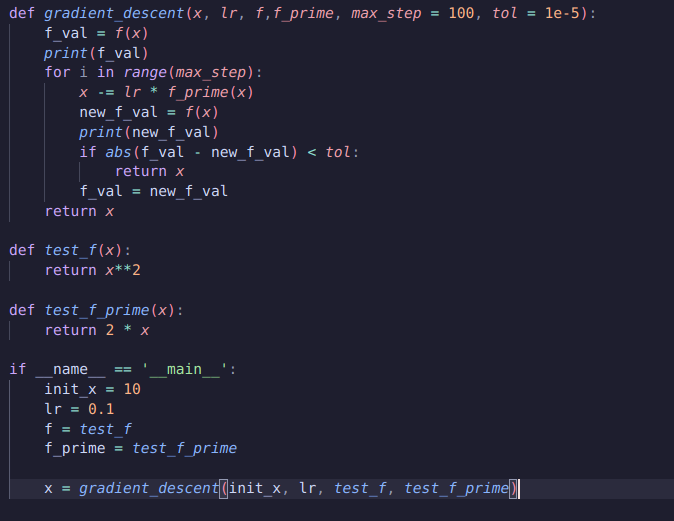
\includegraphics[width=0.72\linewidth]{image/code.png}
    \caption{GD Implementation}
    \label{fig:code}
\end{figure}

\section{Analysis of learning rate effect}
Here in this section, we could make some small tests on the effect of different learning rate to the final result.

\begin{figure}[H]
    \centering
    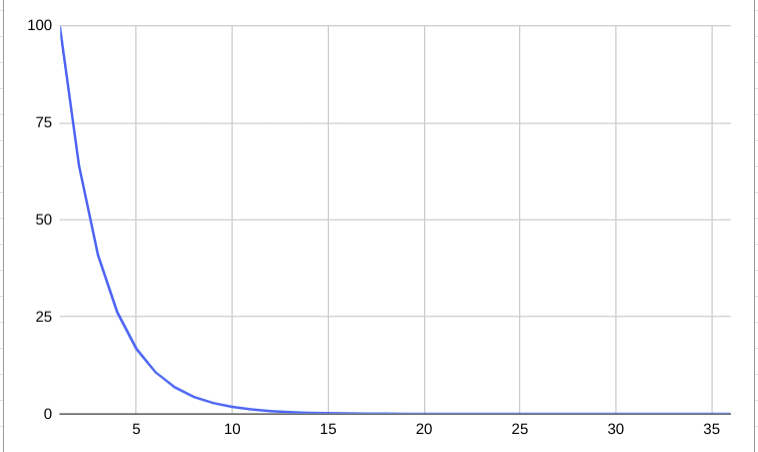
\includegraphics[width=0.75\linewidth]{image/lr01.png}
    \caption{Learning rate = 0.1}
    \label{fig:lr01}
\end{figure}


\begin{figure}[H]
    \centering
    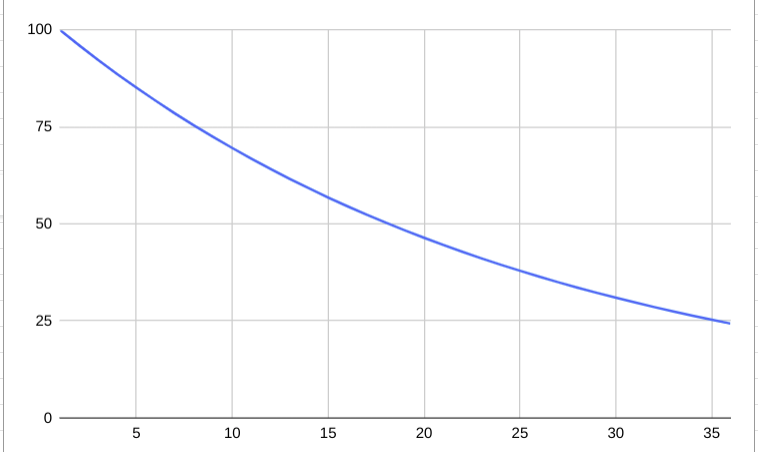
\includegraphics[width=0.75\linewidth]{image/lr001.png}
    \caption{Learning rate = 0.001}
    \label{fig:lr001}
\end{figure}

\begin{figure}[H]
    \centering
    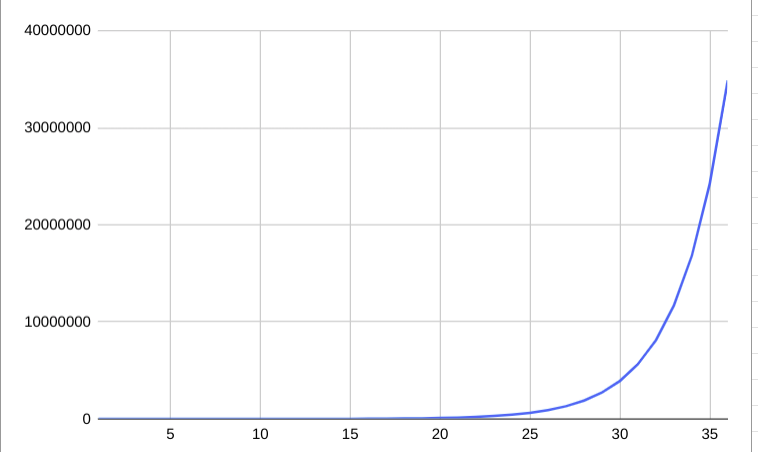
\includegraphics[width=0.75\linewidth]{image/lr11.png}
    \caption{Learning rate = 1.1}
    \label{fig:lr11}
\end{figure}

We make three scenarios according to three different values of learning rate: 0.01, 0.1 and 1.1.
\begin{itemize}
    \item It is clear that with a learning rate of 0.1 shown in figure \ref{fig:lr01}, the model quickly converges in the first few steps and the value become saturated at the end indicating that it's in the minimum value.
    \item With learning rate of 0.01 shown in figure \ref{fig:lr001}, the convergence process occurs much slower. Though the value of the function $f$ still reduces over time, it takes many more step.
    \item With learning rate of 1.1 shown in figure \ref{fig:lr11}, the value increases right in the first few step and continue this trend afterwards. This show the problem of divergence when the learning rate is too huge. 
\end{itemize}
In the end, these experiments show the important of using the correct learning rate for the training process. Else, the final value of $f$ could never converge to the minimal value, or even worse, diverges to huge value.

\end{document}